\documentclass{article}

\def\npart{III}
\def\nyear{2018}
\def\nterm{Michaelmas}
\def\nlecturer{Professor I.\ B.\ Leader}
\def\ncourse{Combinatorics}
\def\draft{Ongoing course, rough}
\ifx \nauthor\undefined
  \def\nauthor{Bhavik Mehta}
\else
\fi

\author{Based on lectures by \nlecturer \\\small Notes taken by \nauthor}
\date{\nterm\ \nyear}
\title{Part \npart\ -- \ncourse}

\usepackage[utf8]{inputenc}
\usepackage{amsmath}
\usepackage{amsthm}
\usepackage{amssymb}
\usepackage{enumerate}
\usepackage{mathtools}
\usepackage{graphicx}
\usepackage[dvipsnames]{xcolor}
\usepackage{tikz}
\usepackage{wrapfig}
\usepackage{centernot}
\usepackage{float}
\usepackage{braket}
\usepackage[hypcap=true]{caption}
\usepackage{enumitem}
\usepackage[colorlinks=true, linkcolor=mblue]{hyperref}
\usepackage[nameinlink,noabbrev]{cleveref}
\usepackage{nameref}
\usepackage[margin=1.5in]{geometry}

% Theorems
\theoremstyle{definition}
\newtheorem*{aim}{Aim}
\newtheorem*{axiom}{Axiom}
\newtheorem*{claim}{Claim}
\newtheorem*{cor}{Corollary}
\newtheorem*{conjecture}{Conjecture}
\newtheorem*{defi}{Definition}
\newtheorem*{eg}{Example}
\newtheorem*{ex}{Exercise}
\newtheorem*{fact}{Fact}
\newtheorem*{law}{Law}
\newtheorem*{lemma}{Lemma}
\newtheorem*{notation}{Notation}
\newtheorem*{prop}{Proposition}
\newtheorem*{question}{Question}
\newtheorem*{rrule}{Rule}
\newtheorem*{thm}{Theorem}
\newtheorem*{assumption}{Assumption}

\newtheorem*{remark}{Remark}
\newtheorem*{warning}{Warning}
\newtheorem*{exercise}{Exercise}

% \newcommand{\nthmautorefname}{Theorem}

\newtheorem{nthm}{Theorem}[section]
\newtheorem{nlemma}[nthm]{Lemma}
\newtheorem{nprop}[nthm]{Proposition}
\newtheorem{ncor}[nthm]{Corollary}
\newtheorem{ndef}[nthm]{Definition}

% Special sets
\newcommand{\C}{\mathbb{C}}
\newcommand{\N}{\mathbb{N}}
\newcommand{\Q}{\mathbb{Q}}
\newcommand{\R}{\mathbb{R}}
\newcommand{\Z}{\mathbb{Z}}

\newcommand{\abs}[1]{\left\lvert #1\right\rvert}
\newcommand{\norm}[1]{\left\lVert #1\right\rVert}
\renewcommand{\vec}[1]{\boldsymbol{\mathbf{#1}}}

\let\Im\relax
\let\Re\relax

\DeclareMathOperator{\Im}{Im}
\DeclareMathOperator{\Re}{Re}
\DeclareMathOperator{\id}{id}

\definecolor{mblue}{rgb}{0., 0.05, 0.6}


% preamble

\setcounter{section}{-1}

\DeclarePairedDelimiter\ceil{\lceil}{\rceil}
\DeclarePairedDelimiter\floor{\lfloor}{\rfloor}

%\newtheorem{manualtheoreminner}{Theorem}
%\newenvironment{manualtheorem}[1]{%
%    \renewcommand\themanualtheoreminner{#1}%
%    \manualtheoreminner
%}{\endmanualtheoreminner}

%\newcommand{\red}[1]{\textcolor{bred}{#1}}
%\newcommand{\green}[1]{\textcolor{bgreen}{#1}}
%\newcommand{\blue}[1]{\textcolor{bblue}{#1}}
%\newcommand{\yellow}[1]{\textcolor{byellow}{#1}}
%\newcommand{\orange}[1]{\textcolor{borange}{#1}}
%\newcommand{\purple}[1]{\textcolor{bpurple}{#1}}

% and here we go!

\begin{document}
\maketitle

\tableofcontents

\clearpage
\section{Introduction}
Combinatorics tends to have problems which are easy to state and hard to prove.
One of the reasons for this is that it is often unclear where to start - for instance in linear algebra we can often start by picking a basis.
Proofs tend to have the property that they seem to take thousands of years to come up with, and a single line to write down.
In this course, we learn some techniques which make problems sounding very hard become very easy.

We start with set systems, which builds on the idea of subsets and containment.
Next, we study isoperimetric inequalities.
In the continuous case, in the plane, a typical problem is to find the maximum area one can enclose with a fixed perimeter, which is solved by a circle.
Similarly, a soap bubble will minimise its surface area for a fixed volume.
Here, in the discrete case, we will try to understand `how tightly' we can pack subsets.
Finally, we look at continuous projections.
For instance, given a subset of space, suppose we know the $z$-coordinate of all points is between $0$ and $1$, and the projection to the $xy$-plane has area $A$, we know the total volume is bounded by $A$.
We generalise this result into higher dimensions and the box result, which has applications in combinatorics.

While all examinable proofs will be included in lectures, relevant books for this course are:
\begin{enumerate}
  \item \emph{Combinatorics}, Bollob\'{a}s, C.U.P., 1996. This matches chapter 1 excellently and parts of chapter 2. It is a gentle read and includes other developments in combinatorics.
  \item \emph{Combinatorics of finite sets}, Anderson, O.U.P., 1987. It is a simple and clear study on chapter 1.
\end{enumerate}

\clearpage
\section{Set systems}
\begin{defi}[Set system]\hypertarget{def:ss}
  Let $X$ be a set. A \textbf{set system} on $X$ (or \textbf{family of subsets} of X) is a family $\mathcal{A} \subseteq \mathcal{P}(X)$.
\end{defi}
For instance, we write $X^{(r)} = \set{A \subset X | |A| = r}$.
Unless otherwise stated, \begin{equation*}X = [n] = \{1,2,\dotsc,n\},\end{equation*} eg $|X^{(r)}| = \binom{n}{r}$.
Thus $[4]^{(2)} = \{12,13,14,23,24,34\}$, so $|[4]^{(2)}| = 6$.

Often, we make $\mathcal{P}(X)$ into a graph, called $Q_n$ by joining $A$ to $B$ if $|A \triangle B| = 1$, i.e.\ if $A = B \cup \{i\}$ for some $i \notin B$ (or vice versa).

For instance, here is a picture of $Q_3$.
\begin{center}
  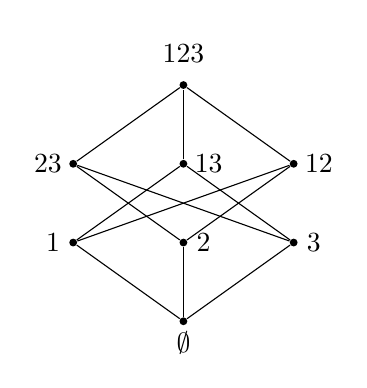
\begin{tikzpicture}[xscale=1.4, every node/.style={fill=black, circle, inner sep=1pt}]
    \node [label=below:$\emptyset$] (empty) at (0,0) {};
    \node [label=left:$1$] (1) at (-1,1) {};
    \node [label=right:$2$] (2) at (0,1) {};
    \node [label=right:$3$] (3) at (1,1) {};
    \node [label=left:$23$] (23) at (-1,2) {};
    \node [label=right:$13$] (13) at (0,2) {};
    \node [label=right:$12$] (12) at (1,2) {};
    \node [label=above:$123$] (123) at (0,3) {};
    \draw (empty) -- (1);
    \draw (empty) -- (2);
    \draw (empty) -- (3);
    \draw (1) -- (12);
    \draw (1) -- (13);
    \draw (2) -- (12);
    \draw (2) -- (23);
    \draw (3) -- (13);
    \draw (3) -- (23);
    \draw (12) -- (123);
    \draw (13) -- (123);
    \draw (23) -- (123);
  \end{tikzpicture}
\end{center}

As we know, the picture gets `thicker' in the middle. But, for odd $n$, is it not clear where exactly the middle is, so in the odd case we have two equally sized large blobs in the middle.

\begin{center}
  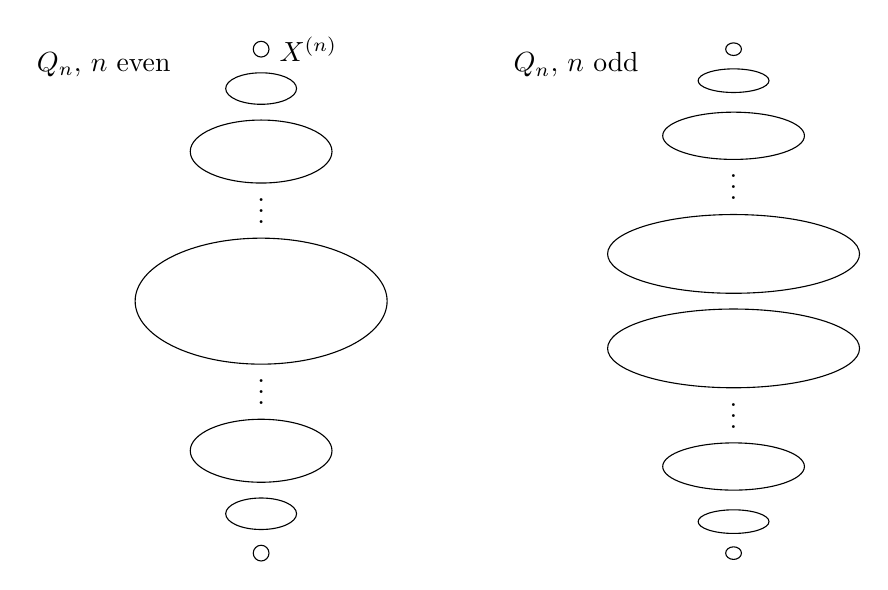
\begin{tikzpicture}
    \begin{scope}
      \node at (-2, 3) {$Q_n$, $n$ even};
      \draw (0,3.2) circle [x radius=1mm, y radius=1mm];
      \draw (0,2.7) circle [x radius=4.5mm, y radius=2mm];
      \draw (0,1.9) circle [x radius=9mm, y radius=4mm];
      \node at (0,1.25) {$\vdots$};
      \draw (0,0) circle [x radius=16mm, y radius=8mm];
      \node at (0,-1.05) {$\vdots$};
      \draw (0,-1.9) circle [x radius=9mm, y radius=4mm];
      \draw (0,-2.7) circle [x radius=4.5mm, y radius=2mm];
      \draw (0,-3.2) circle [x radius=1mm, y radius=1mm];
      \node at (0.6, 3.2) {$X^{(n)}$};
    \end{scope}

    \begin{scope}[xshift=6cm]
      \node at (-2, 3) {$Q_n$, $n$ odd};
      \draw (0,3.2) circle [x radius=1mm, y radius=0.8mm];
      \draw (0,2.8) circle [x radius=4.5mm, y radius=1.5mm];
      \draw (0,2.1) circle [x radius=9mm, y radius=3mm];
      \node at (0,1.55) {$\vdots$};
      \draw (0,0.6) circle [x radius=16mm, y radius=5mm];
      \draw (0,-3.2) circle [x radius=1mm, y radius=0.8mm];
      \draw (0,-2.8) circle [x radius=4.5mm, y radius=1.5mm];
      \draw (0,-2.1) circle [x radius=9mm, y radius=3mm];
      \node at (0,-1.35) {$\vdots$};
      \draw (0,-0.6) circle [x radius=16mm, y radius=5mm];
    \end{scope}
  \end{tikzpicture}
\end{center}
% more pics

If we identify a set $A \subseteq X$ with a $0-1$ sequence of length $n$, e.g.\ $134 \leftrightarrow 1011000\dots0$, via $A \leftrightarrow 1_{A}$ or $\chi_A$, the characteristic function.
Then $Q_3$ looks like
\begin{center}
  \begin{tikzpicture}

  \end{tikzpicture}
\end{center}
\begin{defi}[Hypercube]\hypertarget{def:qn}
  $Q_n$ is often called the \textbf{hypercube} or \textbf{discrete cube} or \textbf{$n$-cube}.
\end{defi}
It is important to keep \emph{both} these pictures in mind: for induction the cube image is more instructive, but when thinking about layers the earlier image is more helpful.

\subsection{Chains and antichains}
\begin{defi}[Chain]\hypertarget{def:chain}
  A family $\mathcal{A} \subseteq \mathcal{P}(X)$ is a \textbf{chain} if $\forall A, B \in \mathcal{A}$, we have $A \subseteq B$ or $B \subseteq A$.
\end{defi}
\begin{defi}[Antichain]\hypertarget{def:antichain}
  A family $\mathcal{A} \subseteq \mathcal{P}(X)$ is an antichain if $\forall A,B \in \mathcal{A}$ with $A \neq B \Rightarrow A \nsubseteq B$.
\end{defi}
\begin{eg}
  For instance, $\{12, 125, 123589\}$ is an \hyperlink{def:chain}{chain}, and $\{1,467,2456\}$ is an \hyperlink{def:antichain}{antichain}.
\end{eg}

In this course, we ask questions like, how large can a \hyperlink{def:chain}{chain} be?
We can achieve $|\mathcal{A}| = n+1$, e.g.\ $\{\emptyset, 1, 12, 123, \dotsc, [n]\}$.
It is easy to visualise this by picking `one per level':

\begin{center}
  \begin{tikzpicture}

  \end{tikzpicture}
\end{center}
We cannot exceed $n+1$, since a chain must meet each `level' $X^{(r)}$ ($0 \leq r \leq n$) in at most one place.

How large can an \hyperlink{def:antichain}{antichain} be?
We could achieve $\mathcal{A}=n$, e.g.\ $\mathcal{A} = \{1,2,3,\dotsc,n\}$ (and this is maximal)
Indeed, could take $\mathcal{A} = X^{(r)}$ for any $r$, so we can achieve $|\mathcal{A}| = \binom{n}{\floor{\frac{n}{2}}}$. Can we beat this?
Aim: Prove this is the winner.
\section{Isoperimetric inequalities}
\section{Projections}
\end{document}
